%%%%%%%%%%%%%%%%%%%%%%%%%%%%%%%%%%%%%%%%%%%%%%%%
% Conectividade em florestas dinamicas         %
%%%%%%%%%%%%%%%%%%%%%%%%%%%%%%%%%%%%%%%%%%%%%%%%
\chapter{Conexidade em florestas dinâmicas}
\label{sec:connDF}

O problema de conexidade em grafos dinâmicos, descrito na Seção \ref{sec:Motivação}, pode ser reduzido ao caso em que o grafo é uma floresta, despertando assim o interesse no \defi[problema!de conexidade em florestas dinâmicas]{problema de conexidade em florestas dinâmicas}. Detalharemos como essa redução é feita no Capítulo~\ref{sec:connDG}. Esse problema pode ser apresentado como a implementação da seguinte biblioteca da forma mais eficiente possível: 

\begin{itemize}
\item \dymForestCreate($n$): cria e retorna uma floresta dinâmica com $n$ vértices isolados;
\item \dymForestAddEdge($F$, $u$, $v$): adiciona a aresta $uv$ à floresta dinâmica~$F$;
\item \dymForestDelEdge($F$, $u$, $v$): remove a aresta $uv$ de $F$; e
\item \dymForestQuery($F$, $u$, $v$): retorna verdadeiro se $u$ e $v$ estão na mesma componente conexa de $F$ e falso, caso contrário.
\end{itemize}
 
Há na literatura uma estrutura de dados bem conhecida chamada \defi{link-cut trees} \cite{SleatroTarjanLinkCutTree1983} que resolve uma versão direcionada desse problema, em que as árvores da floresta são enraizadas.
Com essa estrutura de dados e uma rotina adicional, que permite mudar a raiz de uma dada árvore para um de seus outros nós, as link-cut trees resolvem também a versão não direcionada do problema, ou seja, o problema de conexidade em florestas dinâmicas.
Na Seção~\ref{sec:linkcuttree} introduziremos as link-cut trees como solução para um outro problema envolvendo grafos dinâmicos.
Nessa seção apresentaremos as Euler tour trees, uma solução mais simples e tão eficiente quanto a solução com link-cut trees.


\section{Euler tour trees} 

Tarjan e Vishkin~\cite{tarjan1985} propuseram a \defi{representação por trilha Euleriana} de uma árvore (originalmente chamada de \textit{Euler tour technique}).
Essa representação é obtida de uma árvore~$T$ substituindo-se cada aresta por dois arcos em sentidos opostos e adicionando-se um laço a cada vértice, como pode ser visto na Figura~\ref{fig:exemploSeqEuler}. O digrafo resultante é \defi[grafo!Euleriano]{Euleriano}, ou seja, é conexo e possui uma trilha que começa e termina num mesmo vértice e que passa por todos os arcos do digrafo exatamente uma vez. Uma tal trilha é chamada de \defi{trilha Euleriana} do digrafo.


\begin{figure}[htb]
\centering
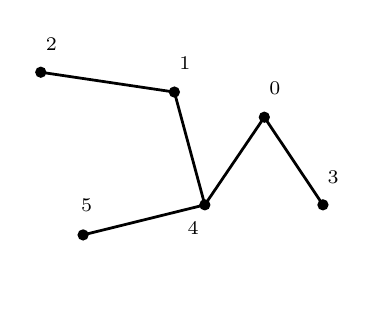
\begin{tikzpicture}[dot/.style={draw,circle,fill,inner sep=1.5pt},line width=1pt,x=1.5cm,y=1.5cm]
\clip(.5,1.3) rectangle (3.3,3.5);
\draw [line width=1pt] (1.7420645075484014,2.9548225063123694)-- (0.6109449986613309,3.1228105521866865);
\draw [line width=1pt] (1.7420645075484014,2.9548225063123694)-- (2,2);
\draw [line width=1pt] (2,2)-- (0.9693194965265414,1.7453085760172875);
\draw [line width=1pt] (2.5036103155119798,2.742037648204901)-- (3,2);
\draw [line width=1pt] (2,2)-- (2.5036103155119798,2.742037648204901);
\begin{scriptsize}
\draw [fill=black,bend left] (1.7420645075484014,2.9548225063123694) circle (1.5pt);
\draw[color=black] (1.8316581320147085,3.195605372065557) node {$1$};
\draw [fill=black] (0.6109449986613309,3.1228105521866865) circle (1.5pt);
\draw[color=black] (0.7005386231276353,3.363593417939874) node {$2$};
\draw [fill=black] (2,2) circle (1.5pt);
\draw[color=black] (1.9,1.8) node {$4$};
\draw [fill=black] (0.9693194965265414,1.7453085760172875) circle (1.5pt);
\draw[color=black] (1,2) node {$5$};
\draw [fill=black] (3,2) circle (1.5pt);
\draw[color=black] (3.0859688745429477,2.2357448368651927) node {$3$};
\draw [fill=black] (2.5036103155119798,2.742037648204901) circle (1.5pt);
\draw[color=black] (2.5932039399782822,2.9828205139580892) node {$0$};
\end{scriptsize}
\end{tikzpicture}

%\documentclass[border=5pt,tikz]{standalone}
%\usetikzlibrary{positioning}
%\begin{document}
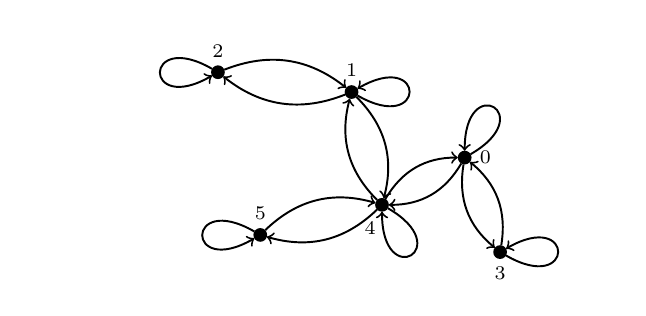
\begin{tikzpicture}[dot/.style={draw,circle,fill,inner sep=1.5pt},line width=.7pt,x=1.5cm,y=1.5cm]
\clip(-1,1.3) rectangle (4,3.5);
\begin{scriptsize}
\node[label=right:0] (r0) at (2.7,2.4) [dot] {};

\node[label=above:1] (r1) at (1.7420645075484014,2.9548225063123694) [dot] {};
%\draw[color=black] (1.8316581320147085,3.195605372065557) node {$1$};


\node[label=above:2] (r2) at (0.6109449986613309,3.1228105521866865) [dot] {};
%\draw[color=black] (0.7005386231276353,3.363593417939874) node {$2$};

\node[label=below:3] (r3) at (3,1.6) [dot] {};
%\draw[color=black] (2.6,1.2357448368651927) node {$3$};

\node (r4) at (2,2) [dot] {};
\draw[color=black] (1.9,1.8) node {$4$};

\node[label=above:5] (r5) at (0.9693194965265414,1.7453085760172875) [dot] {};
%\draw[color=black] (1,2) node {$5$};

\draw[->] (r0) to[out=30,in=90,looseness=30] (r0);
\draw[->] (r1) to[out=-30,in=30,looseness=30] (r1);
\draw[->] (r2) to[out=150,in=210,looseness=30] (r2);
\draw[->] (r3) to[out=-30,in=30,looseness=30] (r3);
\draw[->] (r4) to[out=-30,in=-90,looseness=30] (r4);
\draw[->] (r5) to[out=150,in=210,looseness=30] (r5);

\draw[->] (r0) to[bend left] (r4);
\draw[->] (r4) to[bend left] (r0);

\draw[->] (r0) to[bend right] (r3);
\draw[->] (r3) to[bend right] (r0);

\draw[->] (r5) to[bend left] (r4);
\draw[->] (r4) to[bend left] (r5);

\draw[->] (r1) to[bend left] (r4);
\draw[->] (r4) to[bend left] (r1);

\draw[->] (r1) to[bend left] (r2);
\draw[->] (r2) to[bend left] (r1);

\end{scriptsize}
\end{tikzpicture}
%\end{document}

\caption{Um exemplo de árvore e sua transformação como um digrafo a ser usado para sua representação por trilha Euleriana.}
\label{fig:exemploSeqEuler}
\end{figure}

A representação da árvore~$T$ é essencialmente uma sequência de arcos que forma uma trilha Euleriana de~$T$.
Denotamos cada arco pelo par de vértices que o compõe.
Isto é, o arco com origem no vértice~$u$ e destino no vértice~$v$ é escrito como $uv$.
Dessa forma, um laço em~$v$ é escrito como~$vv$.
Utilizaremos esses laços como representantes dos vértices na sequência. 
Por exemplo, a sequência~\eqref{eq:eulerSeq} é uma trilha Euleriana da árvore da Figura \ref{fig:exemploSeqEuler}.
\begin{equation}
30~00~04~41~12~22~21~11~14~44~45~55~54~40~03~33.\label{eq:eulerSeq}  
\end{equation}

Note que a sequência depende do vértice inicial e da ordem em que cada vizinho de cada vértice é visitado. Chamaremos uma tal sequência de \defi{sequência Euleriana} da árvore~$T$.

Henzinger e King \cite{HenzingerKing} propuseram armazenar uma sequência Euleriana em uma \defi[arvore@\'arvore!binária de busca]{árvore binária de busca} (ABB), que é uma árvore binária composta por nós que possuem  quatro campos: chave, pai, filho esquerdo e filho direito~\cite{CLRS}.

Os campos pai e filhos descrevem a estrutura de árvore binária à ABB. Isto é, cada nó~$N$ possui até dois filhos (esquerdo e direito), o campo \defi{pai} de cada um dos filhos aponta para~$N$. Nenhum nó é filho de dois outros nós. Pode ocorrer de um nó não possuir algum dos filhos; nesse caso, os campos correspondentes a filhos inexistentes contêm~$\Nil$. Somente um nó não possui pai: este é chamado de \defi{raiz} da ABB.

Para uma árvore binária ser considerada de busca, é necessário que, para todo nó $N$, todas as chaves da subárvore esquerda sejam menores do que a chave de $N$ e, simetricamente, todas as chaves da subárvore direita sejam maiores do que a chave de $N$.

Na representação de Henzinger e King, cada nó da ABB guarda um elemento da sequência Euleriana, ou seja, um par de vértices da árvore $T$, em um campo adicional \defi{info}, e armazena, no campo \defi{chave}, um valor entre $1$ e $n$ correspondente ao índice desse elemento na sequência, onde $n$ é o comprimento da sequência.

\begin{figure}[htb]
%\scalebox{.6}{
\centering
\begin{tikzpicture}[line cap=round,line join=round,>=triangle 45,x=1cm,y=1cm]
\clip(-.6,-1) rectangle (14.1,4.6);
\draw [line width=1pt] (1,1) circle (0.5cm);
\draw [line width=1pt] (2,2) circle (0.5cm);
\draw [line width=1pt] (3,1) circle (0.5cm);
\draw [line width=1pt] (5.5,2) circle (0.5cm);
\draw [line width=1pt] (6.5,1) circle (0.5cm);
\draw [line width=1pt] (3.5,3) circle (0.5cm);
\draw [line width=1pt] (7,4) circle (0.5cm);
\draw [line width=1pt] (10.5,3) circle (0.5cm);
\draw [line width=1pt] (9.5,2) circle (0.5cm);
\draw [line width=1pt] (8.5,1) circle (0.5cm);
\draw [line width=1pt] (11.5,2) circle (0.5cm);
\draw [line width=1pt] (10.5,1) circle (0.5cm);
\draw [line width=1pt] (12.5,1) circle (0.5cm);
\draw [line width=1pt] (4.5,1) circle (0.5cm);
\draw [line width=1pt] (7.5,0) circle (0.5cm);
\draw [line width=1pt] (9.5,0) circle (0.5cm);
\draw [line width=1pt] (1.3535533905932737,1.3535533905932737)-- (1.646446609406726,1.646446609406726);
\draw [line width=1pt] (2.353553390593274,1.646446609406726)-- (2.646446609406726,1.353553390593274);
i%\draw [line width=1pt] (2.646446609406726,0.646446609406726)-- (2.353553390593274,0.35355339059327395);
\draw [line width=1pt] (2.416025147168923,2.2773500981126156)-- (3.0839748528310773,2.722649901887385);
\draw [line width=1pt] (3.947213595499958,2.776393202250021)-- (5.052786404500042,2.223606797749979);
\draw [line width=1pt] (5.146446609406726,1.646446609406726)-- (4.853553390593274,1.353553390593274);
\draw [line width=1pt] (5.853553390593274,1.646446609406726)-- (6.146446609406726,1.353553390593274);
\draw [line width=1pt] (10.01923802617959,3.137360563948689)-- (7.480761973820412,3.8626394360513108);
\draw [line width=1pt] (6.519238026179588,3.8626394360513108)-- (3.9807619738204116,3.137360563948689);
\draw [line width=1pt] (10.146446609406727,2.646446609406727)-- (9.853553390593273,2.353553390593273);
\draw [line width=1pt] (9.146446609406727,1.646446609406727)-- (8.853553390593273,1.353553390593273);
\draw [line width=1pt] (8.146446609406727,0.6464466094067269)-- (7.853553390593274,0.35355339059327395);
\draw [line width=1pt] (8.853553390593273,0.6464466094067269)-- (9.146446609406727,0.35355339059327306);
\draw [line width=1pt] (10.853553390593273,1.353553390593273)-- (11.146446609406727,1.646446609406727);
\draw [line width=1pt] (11.146446609406727,2.353553390593273)-- (10.853553390593273,2.646446609406727);
\draw [line width=1pt] (11.853553390593273,1.646446609406727)-- (12.146446609406727,1.353553390593273);


\draw[color=black] (1,1) node {$30$};
\draw[color=black] (1,.2) node {1};
\draw[color=black] (2,2) node {$00$};
\draw[color=black] (2,1.2) node {2};
\draw[color=black] (3,1) node {$04$};
\draw[color=black] (3,.2) node {3};
\draw[color=black] (3.5,3) node {$41$};
\draw[color=black] (3.5,2.2) node {4};
\draw[color=black] (4.5,1) node {$12$};
\draw[color=black] (4.5,.2) node {5};
\draw[color=black] (5.5,2) node {$22$};
\draw[color=black] (5.5,1.2) node {6};
\draw[color=black] (6.5,1) node {$21$};
\draw[color=black] (6.5,.2) node {7};
\draw[color=black] (7,4) node {$11$};
\draw[color=black] (7,3.2) node {8};
\draw[color=black] (7.5,0) node {$14$};
\draw[color=black] (7.5,-.8) node {9};
\draw[color=black] (8.5,1) node {$44$};
\draw[color=black] (8.5,.2) node {10};
\draw[color=black] (9.5,0) node {$45$};
\draw[color=black] (9.5,-.8) node {11};
\draw[color=black] (9.5,2) node {$55$};
\draw[color=black] (9.5,1.2) node {12};
\draw[color=black] (10.5,3) node {$54$};
\draw[color=black] (10.5,2.2) node {13};
\draw[color=black] (10.5,1) node {$40$};
\draw[color=black] (10.5,.2) node {14};
\draw[color=black] (11.5,2) node {$03$};
\draw[color=black] (11.5,1.2) node {15};
\draw[color=black] (12.5,1) node {$33$};
\draw[color=black] (12.5,.2) node {16};


\end{tikzpicture}
%}
\caption{Sequência~\eqref{eq:eulerSeq}  armazenada em uma ABB. Dentro do círculo mostramos o arco armazenado no nó e abaixo do círculo está sua chave.}
\label{fig:seq-treap-indices}
\end{figure}

Por exemplo, a ABB na Figura~\ref{fig:seq-treap-indices} está armazenando a sequência Euleriana~\eqref{eq:eulerSeq}.
Uma tal ABB é chamada de \defi{Euler tour tree}. 
Henzinger e King propuseram representar uma floresta por uma coleção de Euler tour trees: uma para cada componente da floresta. 
Dessa forma, como veremos na Seção~\ref{sec:impleDF-ETT}, é possível obter uma implementação de uma floresta dinâmica em que as operações de consulta de conexidade e de inserção e remoção de aresta têm consumo esperado~$\O{\lg n}$, onde $n$ é o número de vértices da floresta.


\section{Implementação de floresta dinâmica com Euler tour trees}
\label{sec:impleDF-ETT}

Para implementar a biblioteca de florestas dinâmicas com Euler tour trees, consideremos inicialmente a seguinte biblioteca.

\begin{itemize}
\item  \treapCreate($u$, $v$): cria e retorna uma ABB com somente um nó que armazena o par de vértices $uv$;
\item \treapGetRoot($\node$): retorna a raiz da ABB que contém $\node$;
\end{itemize}

A implementação dessas rotinas será detalhada no Capítulo~\ref{sec:TreapDeChaveImplicita}. Veremos que o consumo esperado de \treapCreate{} e \treapGetRoot{} será, respectivamente,~$\O{1}$ e~$\O{\lg n}$, onde~$n$ é o número de nós na ABB.

Para representar uma floresta dinâmica $F$, precisaremos também de um dicionário que guardará apontadores para os nós das Abbs que representam~$F$. Note que cada nó representa um elemento $uv$ de uma sequência Euleriana e que cada~$uv$ ocorre no máximo uma vez nas sequências. Entao o par $(u,v)$ será usado como chave e o valor correspondente a tal chave será o apontador para o nó que contém $uv$ nas ABBs que representam~$F$.

Para simplificar os pseudo-códigos, usaremos uma representação matricial para esse dicionário, ou seja, usaremos a seguinte biblioteca.
\begin{itemize}
    \item $F \gets \hashCreate(n)$: cria e retorna um dicionário~$F$ para uma floresta dinâmica com~$n$ vértices;
    \item $F[u,v] \gets uv$: insere o nó que contém $uv$, com chave $(u,v)$ e valor associado~$uv$ na tabela~$F$.
    Se o par~$(u,v)$ já estiver presente no dicionário, então seu valor associado é substituído por~$uv$;
    \item $F[u,v] \gets \Nil{}$: remove o nó associado ao~$(u,v)$ e seu valor associado do dicionário~$F$;
    \item $\var \gets F[u,v]$: atribui o valor associado à chave~$(u,v)$ à variável~$\var$; Caso a chave~$(u,v)$ não esteja presente em~$F$, atribui~$\Nil$ a~$\var$.
\end{itemize}
Existem implementações bem conhecidas de dicionários em que a primeira rotina consome~$\O{n}$ e as demais consomem tempo esperado~$\O{1}$~\cite{CLRS}.

No Algoritmo~\ref{Algo:dymForestCreate} apresentamos a implementação de~\dymForestCreate{}, que cria e retorna uma nova floresta dinâmica que possui $n$ vértices e nenhuma aresta.
Já no Algoritmo~\ref{Algo:dymForestQuery} mostramos a implementação de~\dymForestQuery{}, que responde à consulta de conexidade entre dois vértices~$u$ e~$v$ na floresta~$F$.


\begin{algorithm}[htb]
\caption{\dymForestCreate($n$)}
\label{Algo:dymForestCreate}
\begin{algorithmic}[1]
\State $F~\gets~\hashCreate(n)$
\For {$v$ $\gets$ 1 até $n$}\label{Algo:dymForestCreate:for}
\State $F[v,v]~\gets$ \treapCreate($v$, $v$)
\EndFor
\State \Return $F$
\end{algorithmic}
\end{algorithm}

Com essa implementação \dymForestCreate{} consume tempo~$\O{n}$. A rotina \dymForestQuery{}, descrita no Algoritmo~\ref{Algo:dymForestQuery}, consume tempo esperado $\O{\lg n}$ em uma floresta com~$n$ vértices.


\begin{algorithm}[htb]
\caption{\dymForestQuery($F$, $u$, $v$)}
\label{Algo:dymForestQuery}
\begin{algorithmic}[1]
\State $uu$ $\gets$ $F[u,u]$
\State $\mathit{uu}$ $\gets$ $F[u,u]$
\State $vv$ $\gets$ $F[v,v]$
\State $\mathit{vv}$ $\gets$ $F[v,v]$
\State \Return \treapGetRoot($uu$) = \treapGetRoot($vv$)
\end{algorithmic}
\end{algorithm}

Para implementar \dymForestAddEdge{} e \dymForestDelEdge{}, precisaremos adicionalmente das seguintes rotinas na biblioteca de Euler tour trees. 
\begin{itemize}
\NEW{
\item \treapSplit($\node$): recebe um ponteiro para um nó~$\node$ e corta a ABB que contém esse nó em três ABBs. A primeira ABB contém todos os nós com chave estritamente menor do que a chave de~$\node$, a segunda contém somente~$\node$ e a última contém todos os nós com chave estritamente maior do que a chave de~$\node$. Essa rotina retorna as raízes dessas três ABBs; e
}
\item \treapJoin($T_1, T_2, \ldots, T_k$): junta as ABBs $T_1, T_2, \ldots, T_{k-1}$ e $T_k$ de modo que a sequência armazenada na árvore resultante é a concatenação das sequências armazenada em~$T_1, T_2, \ldots, T_k$ e retorna a raiz dessa árvore resultante.
\end{itemize}

Na Seção~\ref{sec:imple-treap}, mostraremos a implementação dessas rotinas e que~\treapJoin{} consome~$\O{h}$, onde~$h$ é a soma das alturas de~$T_1, T_2, \ldots, T_k$ e \treapSplit{} consome~$\O{\lg n}$, onde~$n$ é número de nós da árvore que contém~$\node$.

Para implementar a operação \dymForestDelEdge($F$, $u$, $v$), descrita no Algoritmo~\ref{Algo:dymForestDelEdge}, 
primeiro utilizaremos o dicionário para obter ponteiros para os nós que armazenam os arcos $uv$ e $vu$.

Em seguida, aplicaremos~\treapSplit($uv$) dividindo essa sequência em duas partes, nomeadas~$A$ e~$B$, como pode ser visto na Figura~\ref{fig:algorit-cut-seqxy}.
\begin{figure}[htb]
\centering
\definecolor{ccqqqq}{rgb}{1,0,0}
\definecolor{qqqqcc}{rgb}{0,0,1}
\begin{tikzpicture}[line cap=round,line join=round,>=triangle 45,x=1cm,y=1cm]
\clip(-.1,-.6) rectangle (10.1,1.1);
\draw (-.1,0.8) node[anchor=north west] {\Large $w$};
\draw [line width=1pt] (0,0)-- (3,0);
\draw [line width=1pt] (0,1)-- (3,1);

\draw [line width=1pt] (0,0)-- (0,1);
\draw (2.45,0.8) node[anchor=north west] {\Large $u$};
\draw [line width=1pt] (3,1)-- (3,0);
\draw (1.2,0.85) node[anchor=north west] {\Large $A$};


\draw (4.05,0.8) node[anchor=north west] {\Large $uv$};
\draw [line width=1pt] (4,0)-- (5,0);
\draw [line width=1pt] (4,1)-- (5,1);
\draw [line width=1pt] (5,1)-- (5,0);
\draw [line width=1pt] (4,1)-- (4,0);


\draw [line width=1pt] (6,0)-- (6,1);
\draw [line width=1pt] (6,0)-- (10,0);
\draw [line width=1pt] (6,1)-- (10,1);
\draw [line width=1pt] (10,1)-- (10,0);
\draw (9.3,0.8) node[anchor=north west] {\Large $w$};

\draw (6.05,0.8) node[anchor=north west] {\Large $v$};
\draw (7.5,0.85) node[anchor=north west] {\Large $B$};
\end{tikzpicture}

\caption{Sequências $A$ e $B$ após a chamada de \treapSplit($uv$).}
\label{fig:algorit-cut-seqxy}
\end{figure}

Como a sequência original é Euleriana, sabemos que o primeiro e último vértice dessa sequência coincidem. Na Figura~\ref{fig:algorit-cut-seqxy} chamamos esse vértice de~$w$.
Dessa forma~$A$ representa uma trilha de~$w$ até~$u$ e~$B$ representa uma trilha de~$v$ até~$w$.

Note que não sabemos se $vu$ está na sequência~$A$ ou na sequência~$B$, mas não precisaremos dessa informação, pois podemos fazer a concatenação de~$B$ com~$A$,
chamando \treapJoin($B$, $A$), obtendo uma trilha de~$v$ até~$u$ que passa pelo arco~$vu$ em algum ponto.

Por fim, para concluir esse algoritmo, basta chamar~\treapSplit($vu$) para dividir essa sequência em duas.
A primeira sendo a sequência Euleriana que representa a árvore que contém o vértice~$v$ e a segunda sendo a sequência Euleriana que contém o vértice~$u$.

\begin{algorithm}[htb]
\caption{\dymForestDelEdge($F$, $u$, $v$)}
\label{Algo:dymForestDelEdge}
\begin{algorithmic}[1]
\State $uv$ $\gets$ $F[u,v]$\label{Algo:dymForestDelEdge:1}
\State $vu$ $\gets$ $F[v,u]$\label{Algo:dymForestDelEdge:2}
\State $A$, $uv$, $B$ $\gets$ \treapSplit($uv$)\label{Algo:dymForestDelEdge:3}
\State \treapJoin($B$, $A$)\label{Algo:dymForestDelEdge:4}
\State \treapSplit($vu$)\label{Algo:dymForestDelEdge:5}
\State $F[u,v]$ $\gets$ $\Nil{}$\label{Algo:dymForestDelEdge:6}
\State $F[v,u]$ $\gets$ $\Nil{}$\label{Algo:dymForestDelEdge:7}
\end{algorithmic}
\end{algorithm}

\NEW{
Notemos que as linhas~\ref{Algo:dymForestDelEdge:1},~\ref{Algo:dymForestDelEdge:2},~\ref{Algo:dymForestDelEdge:6} e~\ref{Algo:dymForestDelEdge:7} do Algoritmo~\ref{Algo:dymForestDelEdge} consumem tempo esperado constante.
Enquanto que as linhas~\ref{Algo:dymForestDelEdge:3},~\ref{Algo:dymForestDelEdge:4} e~\ref{Algo:dymForestDelEdge:5}, e consequentemente \dymForestDelEdge{}, possuem consumo de tempo~$\O{\lg n}$, onde~$n$ é o número de vértices de~$F$.
}

Como exemplo, veremos o que ocorre com a sequência~\eqref{eq:eulerSeq} durante a execução da chamada \dymForestDelEdge($F$, $1$, $4$).
Primeiro, após a chamada de \treapSplit($14$), obtemos árvores correspondentes às seguinte duas sequências:
\begin{equation}
A = 30~00~04~41~12~22~21~11~~~~~~~~~~~~B = 44~45~55~54~40~03~33.\nonumber
\end{equation}
Nesse caso, temos que $w=3$. Após \treapJoin($B$, $A$), temos uma árvore que representa a sequência
\begin{equation}
 44~45~55~54~40~03~33~30~00~04~41~12~22~21~11.\nonumber
\end{equation}
Por fim, após \treapSplit($41$), temos árvores que representam as duas sequências
\begin{equation}
 44~45~55~54~40~03~33~30~00~04~~~~~\text{e}~~~~~~12~22~21~11.\label{eq:apos-remocao}
\end{equation}
Note que as duas sequências resultantes representam a floresta obtida pela remoção da aresta~$14$, que está ilustrada na Figura~\ref{fig:algorit-del-pos}.

\begin{figure}[htb]
\centering
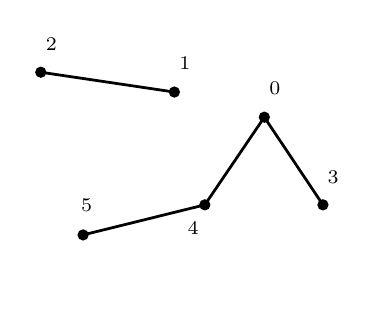
\begin{tikzpicture}[dot/.style={draw,circle,fill,inner sep=1.5pt},line width=1pt,x=1.5cm,y=1.5cm]
\clip(.5,1.3) rectangle (3.3,3.5);
\draw [line width=1pt] (1.7420645075484014,2.9548225063123694)-- (0.6109449986613309,3.1228105521866865);
%\draw [line width=1pt] (1.7420645075484014,2.9548225063123694)-- (2,2);
\draw [line width=1pt] (2,2)-- (0.9693194965265414,1.7453085760172875);
\draw [line width=1pt] (2.5036103155119798,2.742037648204901)-- (3,2);
\draw [line width=1pt] (2,2)-- (2.5036103155119798,2.742037648204901);
\begin{scriptsize}
\draw [fill=black,bend left] (1.7420645075484014,2.9548225063123694) circle (1.5pt);
\draw[color=black] (1.8316581320147085,3.195605372065557) node {$1$};
\draw [fill=black] (0.6109449986613309,3.1228105521866865) circle (1.5pt);
\draw[color=black] (0.7005386231276353,3.363593417939874) node {$2$};
\draw [fill=black] (2,2) circle (1.5pt);
\draw[color=black] (1.9,1.8) node {$4$};
\draw [fill=black] (0.9693194965265414,1.7453085760172875) circle (1.5pt);
\draw[color=black] (1,2) node {$5$};
\draw [fill=black] (3,2) circle (1.5pt);
\draw[color=black] (3.0859688745429477,2.2357448368651927) node {$3$};
\draw [fill=black] (2.5036103155119798,2.742037648204901) circle (1.5pt);
\draw[color=black] (2.5932039399782822,2.9828205139580892) node {$0$};
\end{scriptsize}
\end{tikzpicture}

\caption{Floresta resultante de~\dymForestDelEdge($F$, $1$, $4$), representada pelas sequências em~\eqref{eq:apos-remocao}.}
\label{fig:algorit-del-pos}
\end{figure}

Para implementar \dymForestAddEdge{}, descrita no Algoritmo~\ref{Algo:dymForestAddEdge}, utilizamos a rotina auxiliar \ETmovetofront{}.
Essa rotina recebe uma floresta~$F$ e um vértice~$u$ e restrutura a ABB que contém $uu$ de forma que este se torne o primeiro elemento de sua sequência Euleriana, e retorna a raiz da ABB resultante. 

Por exemplo, se aplicarmos \ETmovetofront($F$,2) e \ETmovetofront($F$,5), onde $F$ é a floresta dinâmica ilustrada na Figura~\ref{fig:algorit-del-pos}, obtemos as sequências:
\begin{equation}
55~54~40~03~33~30~00~04~44~45~~~~~\text{e}~~~~~~22~21~11~12.\label{eq:apos-moveToFront}
\end{equation}

Para implementar~\ETmovetofront($F$, $u$), basta cortar a sequência em $uu$ chamando \treapSplit($uu$) e concatenar as sequências resultantes de forma apropriada com~\treapJoin{}.
Note que, como \treapSplit{} remove $uu$ da sequência, temos que adicioná-lo novamente à sequência como pode ser visto na linha~\ref{Algo:Etmovetofront:linha3} do Algoritmo~\ref{Algo:ETmovetofront}.

\begin{algorithm}[htb]
\caption{\ETmovetofront($F$, $u$)}
\label{Algo:ETmovetofront}
\begin{algorithmic}[1]
\State $uu$ $\gets$ $F[u,u]$\label{Algo:ETmovetofront:1}
\State $A$, $uu$, $B$ $\gets$ \treapSplit($uu$)\label{Algo:ETmovetofront:2}
\State \Return \treapJoin($uu$, $B$, $A$)\label{Algo:ETmovetofront:linha3}\label{Algo:ETmovetofront:3}
\end{algorithmic}
\end{algorithm}

\NEW{
Notemos que, devido às linhas~\ref{Algo:ETmovetofront:2} e~\ref{Algo:ETmovetofront:3} do Algoritmo~\ref{Algo:ETmovetofront}, o consumo de tempo de \ETmovetofront{} é $\O{\lg n}$.
}
Com a rotina \ETmovetofront{} implementada, podemos elaborar~\dymForestAddEdge{}, descrita no Algoritmo~\ref{Algo:dymForestAddEdge}.


\begin{algorithm}[htb]
\caption{\dymForestAddEdge($F$, $u$, $v$)}
\label{Algo:dymForestAddEdge}
\begin{algorithmic}[1]
\State $U$ $\gets$ \ETmovetofront($F$, $u$)
\State $V$ $\gets$ \ETmovetofront($F$, $v$)
\State $uv$ $\gets$ \treapCreate($u$, $v$)
\State $vu$ $\gets$ \treapCreate($v$, $u$)
\State $F[u,v]$ $\gets$ $uv$
\State $F[v,u]$ $\gets$ $vu$
\State \treapJoin($U$, $uv$, $V$, $vu$)
\end{algorithmic}
\end{algorithm}

Primeiro, usamos \ETmovetofront{} para mover~$uu$ e~$vv$ para o início de suas sequências.
Em seguida, criamos novos nós~$uv$ e~$vu$; os adicionamos à tabela de símbolos e usamos \treapJoin{} pra unir todas as sequências de tal forma que a sequência resultante seja a sequência Euleriana correspondente a árvore resultante da adição da aresta~$uv$.

Dessa forma, se quisermos adicionar uma aresta ligando os vértices~$2$ e~$5$ na floresta da Figura~\ref{fig:algorit-del-pos}, obtendo assim a floresta da Figura~\ref{fig:algorit-add-pos}, primeiro temos que mover $22$ e $55$ para o início de suas sequências, como fizemos com as sequências \eqref{eq:apos-moveToFront}. Em seguida criamos os nós contendo $25$ e $52$ e unimos essas sequências, obtendo assim a sequência:
\begin{equation}
55~54~40~03~33~30~00~04~44~45~52~22~21~11~12~25.\label{eq:add}
\end{equation}
Logo, o consumo esperado de \dymForestAddEdge{} também será~$\O{\lg n}$.

\begin{figure}[htb]
\centering
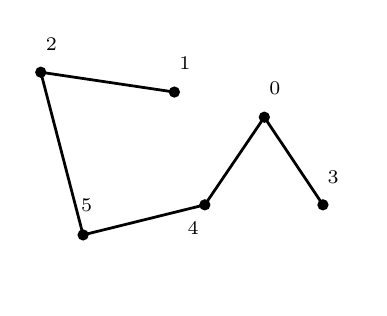
\begin{tikzpicture}[dot/.style={draw,circle,fill,inner sep=1.5pt},line width=1pt,x=1.5cm,y=1.5cm]
\clip(.5,1.3) rectangle (3.3,3.5);
\draw [line width=1pt] (1.7420645075484014,2.9548225063123694)-- (0.6109449986613309,3.1228105521866865);
\draw [line width=1pt] (2,2)-- (0.9693194965265414,1.7453085760172875);
\draw [line width=1pt] (2.5036103155119798,2.742037648204901)-- (3,2);
\draw [line width=1pt] ( 0.9693194965265414,1.7453085760172875         )-- (0.6109449986613309,3.1228105521866865  );
\draw [line width=1pt] (2,2)-- (2.5036103155119798,2.742037648204901);
\begin{scriptsize}
\draw [fill=black,bend left] (1.7420645075484014,2.9548225063123694) circle (1.5pt);
\draw[color=black] (1.8316581320147085,3.195605372065557) node {$1$};
\draw [fill=black] (0.6109449986613309,3.1228105521866865) circle (1.5pt);
\draw[color=black] (0.7005386231276353,3.363593417939874) node {$2$};
\draw [fill=black] (2,2) circle (1.5pt);
\draw[color=black] (1.9,1.8) node {$4$};
\draw [fill=black] (0.9693194965265414,1.7453085760172875) circle (1.5pt);
\draw[color=black] (1,2) node {$5$};
\draw [fill=black] (3,2) circle (1.5pt);
\draw[color=black] (3.0859688745429477,2.2357448368651927) node {$3$};
\draw [fill=black] (2.5036103155119798,2.742037648204901) circle (1.5pt);
\draw[color=black] (2.5932039399782822,2.9828205139580892) node {$0$};
\end{scriptsize}
\end{tikzpicture}

\caption{Floresta resultante de~\dymForestAddEdge($F$, $2$, $5$), representada pelas sequências~\eqref{eq:add}.}
\label{fig:algorit-add-pos}
\end{figure}
